\iffalse
\chapter{2022}
\author{EE24BTECH11059}
\section{ae}
\fi
    %code by ysiddhanth 
	\item{
		Q.1 Writing too many things on the \underline{ \hspace{1.5cm}} while teaching could make the students get \underline{ \hspace{1.5cm}     }.
		\begin{enumerate}
			\begin{multicols}{4}
				\item bored / board
				\item board / bored
				\item board / board
				\item bored / bored
			\end{multicols}
		\end{enumerate}
	}
	\item{
        	
        	Which one of the following is a representation (not to scale and in bold) of all values of \(x\) satisfying the inequality \(2 - 5x \le -\frac{6x-5}{3}\) on the real number line?
        	\begin{enumerate}
        			\item{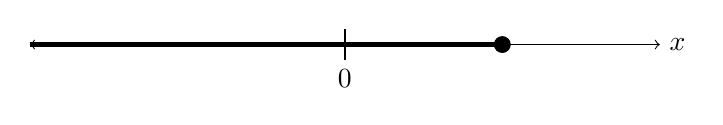
\begin{tikzpicture}
        					% Draw the entire x-axis
        					\draw[<->] (-4, 0) -- (4, 0);
        					
        					% Draw the thick segment
        					\draw[ultra thick] (-4, 0) -- (2, 0);
        					
        					% Mark the origin
        					\draw[thick] (0, -0.2) -- (0, 0.2);
        					\node[below] at (0, -0.2) {0};
        					
        					% Draw the filled circle
        					\filldraw[black] (2, 0) circle (0.1);
        					
        					% Label the x-axis
        					\node[right] at (4, 0) {$x$};
        					
        			\end{tikzpicture}}
        		\item{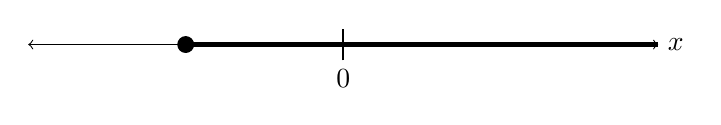
\begin{tikzpicture}
        				% Draw the entire x-axis
        				\draw[<->] (-4, 0) -- (4, 0);
        				
        				% Draw the thick segment
        				\draw[ultra thick] (-2, 0) -- (4, 0);
        				
        				% Mark the origin
        				\draw[thick] (0, -0.2) -- (0, 0.2);
        				\node[below] at (0, -0.2) {0};
        				
        				% Draw the filled circle
        				\filldraw[black] (-2, 0) circle (0.1);
        				
        				% Label the x-axis
        				\node[right] at (4, 0) {$x$};
        				
        		\end{tikzpicture}}
        	\item{\begin{tikzpicture}
        			% Draw the entire x-axis
        			\draw[<->] (-4, 0) -- (4, 0);
        			
        			% Draw the thick segment
        			\draw[ultra thick] (2, 0) -- (4, 0);
        			
        			% Mark the origin
        			\draw[thick] (0, -0.2) -- (0, 0.2);
        			\node[below] at (0, -0.2) {0};
        			
        			% Draw the filled circle
        			\filldraw[black] (2, 0) circle (0.1);
        			
        			% Label the x-axis
        			\node[right] at (4, 0) {$x$};
        			
        	\end{tikzpicture}}
        \item{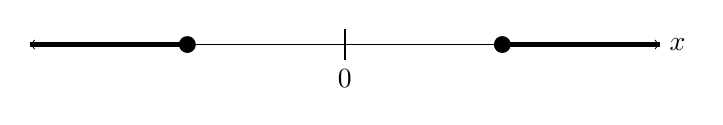
\begin{tikzpicture}
        		% Draw the entire x-axis
        		\draw[<->] (-4, 0) -- (4, 0);
        		
        		% Draw the thick segment
        		\draw[ultra thick] (-2, 0) -- (-4, 0);
        		\draw[ultra thick] (2, 0) -- (4, 0);
        		
        		% Mark the origin
        		\draw[thick] (0, -0.2) -- (0, 0.2);
        		\node[below] at (0, -0.2) {0};
        		
        		% Draw the filled circle
        		\filldraw[black] (-2, 0) circle (0.1);
        		\filldraw[black] (2, 0) circle (0.1);
        		
        		% Label the x-axis
        		\node[right] at (4, 0) {$x$};
        		
        \end{tikzpicture}}
        	\end{enumerate}
        	
      }
        \item {
        	If \( f(x) = 2 \ln(\sqrt{e^x}) \), what is the area bounded by \( f(x) \) for the interval \([0, 2]\) on the \( x \)-axis?
        	\begin{enumerate}
        		\begin{multicols}{4}
        			\item \( \frac{1}{2} \) \\
        			\item \( 1 \) \\
        			\item \( 2 \) \\
        			\item \( 4 \)
        		\end{multicols}
        	\end{enumerate}
  		}
    
    \item {
    	The point of maximum entropy on a Fanno-curve in a Temperature-Entropy (T-s)
    	diagram represents the 
    	\begin{multicols}{2}
	    	\begin{enumerate}
	    		\item maximum flow Mach number
	    		\item minimum flow Mach number
	    		\item sonic Mach number
	    		\item normal shock in the flow 
	    	\end{enumerate}
	    \end{multicols}
    
    }    
    \item {A three-member committee has to be formed from a group of 9 people. How many such distinct committees can be formed? (tikz)
    	\begin{multicols}{4}
	    	\begin{enumerate}
	    		\item 27
	    		\item 72
	    		\item 81
	    		\item 84
	    	\end{enumerate}
    	\end{multicols}}
    \item {
    	Fish belonging to species S in the deep sea have skins that are extremely black
    	(ultra-black skin). This helps them not only to avoid predators but also sneakily
    	attack their prey. However, having this extra layer of black pigment results in
    	lower collagen on their skin, making their skin more fragile. \\
    	Which one of the following is the CORRECT logical inference based on the
    	information in the above passage? 
    		\begin{enumerate}
    			\item Having ultra-black skin is only advantageous to species S
    			\item Species S with lower collagen in their skin are at an advantage because it helps
    			them avoid predators
    			\item Having ultra-black skin has both advantages and disadvantages to species S
    			\item Having ultra-black skin is only disadvantageous to species S but advantageous
    			only to their predators 
    		\end{enumerate}
	}
    \item {
    	For the past $m$ days, the average daily production at a company was 100 units
    	per day.
    	If today’s production of 180 units changes the average to 110 units per day,
    	what is the value of $m$? 
    	
    	
    	\begin{multicols}{4}
    		\begin{enumerate}
    			\item 18
    			\item 10 
    			\item 7
    			\item 5
    		\end{enumerate}
    	\end{multicols}
    
	}
    \item{
            Consider the following functions for non-zero positive integers, \(p\) and \(q\).
            \[
            f(p, q) = \underbrace{p \times p \times p \times \dots \times p}_{q \text{ terms}} = p^q; \quad f(p, 1) = p
            \]
            \[
            g(p, q) = p^{p^{p^{p^{p^{.^{.^{.^{\text{Upto q terms}}}}}}}}}; \quad g(p, 1) = p
            \]
            Which one of the following options is correct based on the above?
            
            
                
            \begin{multicols}{2}
                \begin{enumerate}
                	\item \(f(2,2) = g(2,2)\) \\
                	\item \(f(g(2,2), 2) < f(2, g(2,2))\) \\
                	\item \(g(2,1) \ne f(2,1)\) \\
                	\item \(f(3,2) > g(3,2)\)
                \end{enumerate}
            \end{multicols}

        %code by ysiddhanth 
        
        }
    \item{
            Four cities P, Q, R and S are connected through one-way routes as shown in the
            figure. The travel time between any two connected cities is one hour. The boxes
            beside each city name describe the starting time of first train of the day and their
            frequency of operation. For example, from city P, the first trains of the day start
            at 8 AM with a frequency of 90 minutes to each of R and S. A person does not
            spend additional time at any city other than the waiting time for the next
            connecting train. \\ 
            If the person starts from R at 7 AM and is required to visit S and return to R,
            what is the minimum time required?
          \begin{center}
          	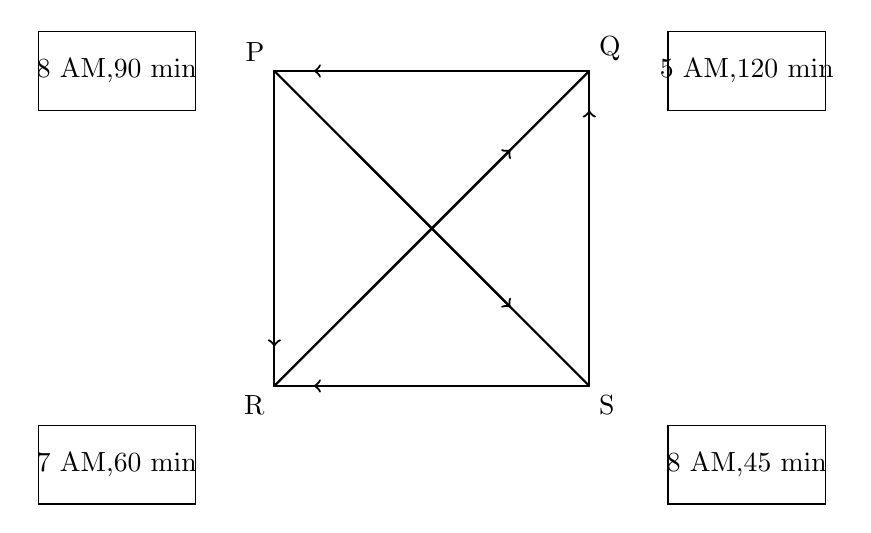
\begin{tikzpicture}
          		
          		% Coordinates for the square and text boxes
          		\coordinate (P) at (0,4);
          		\coordinate (Q) at (4,4);
          		\coordinate (R) at (0,0);
          		\coordinate (S) at (4,0);
          		
          		% Drawing the square
          		\draw[thick] (P) -- (Q) -- (S) -- (R) -- cycle;
          		\draw[thick] (P) -- (S); % Diagonal
          		\draw[thick] (R) -- (Q); % Diagonal
          		
          		% Arrows on edges
          		\draw[->, thick] (3.5,4) -- (0.5,4); % P to Q
          		\draw[->, thick] (0,3.5) -- (0,0.5); % P to R
          		\draw[->, thick] (4,0.5) -- (4,3.5); % Q to S
          		\draw[->, thick] (3.5,0) -- (0.5,0); % R to S
          		
          		% Arrows on diagonals
          		\draw[->, thick] (1,3) -- (3,1); % P to S
          		\draw[->, thick] (1,1) -- (3,3); % Q to R
          		
          		% Labels for corners
          		\node[above left] at (P) {P};
          		\node[above right] at (Q) {Q};
          		\node[below left] at (R) {R};
          		\node[below right] at (S) {S};
          		
          		% Time and duration boxes
          		\draw (P) ++(-1,0.5) rectangle ++(-2,-1) node[pos=.5] {8 AM,90 min};
          		\draw (Q) ++(1,0.5) rectangle ++(2,-1) node[pos=.5] {5 AM,120 min};
          		\draw (R) ++(-1,-0.5) rectangle ++(-2,-1) node[pos=.5] {7 AM,60 min};
          		\draw (S) ++(1,-0.5) rectangle ++(2,-1) node[pos=.5] {8 AM,45 min};
          		
          	\end{tikzpicture}
          \end{center}
            \begin{enumerate}
            	\begin{multicols}{2}
            		\item 6 hours 30 minutes
            		\item 3 hours 45 minutes
            		\item 4 hours 30 minutes
            		\item 5 hours 15 minutes 
            	\end{multicols}
            \end{enumerate}
        
        }
    \item{
           Equal sized circular regions are shaded in a square sheet of paper of 1 cm side
           length. Two cases, case M and case N, are considered as shown in the figures
           below. In the case M, four circles are shaded in the square sheet and in the case
           N, nine circles are shaded in the square sheet as shown.
           What is the ratio of the areas of unshaded regions of case M to that of case N?  
           \begin{center}
           		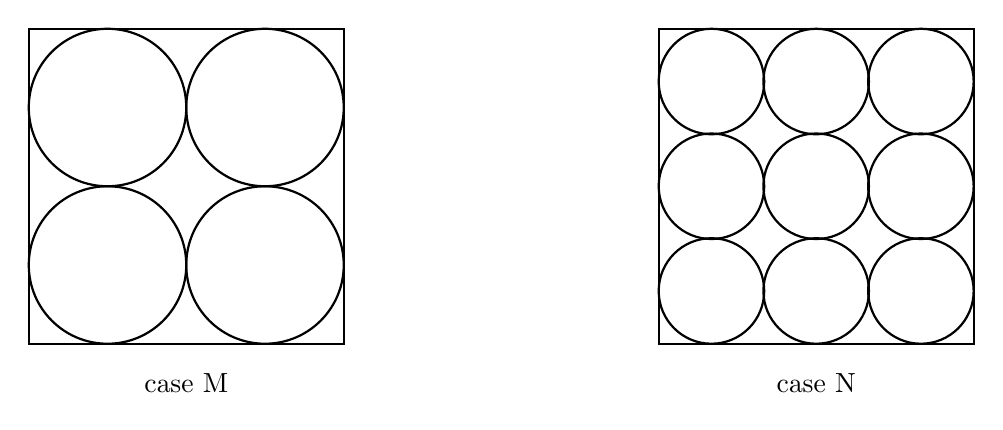
\begin{tikzpicture}
           			% Case M
           			\begin{scope}[shift={(-6, 0)}]
           				% Outer square
           				\draw[thick] (0, 0) rectangle (4, 4);
           				% Circles
           				\foreach \x in {1, 3} {
           					\foreach \y in {1, 3} {
           						\draw[thick] (\x, \y) circle (1);
           					}
           				}
           				\node at (2, -0.5) {case M};
           			\end{scope}
           			
           			% Case N
           			\begin{scope}[shift={(2, 0)}]
           				% Outer square
           				\draw[thick] (0, 0) rectangle (4, 4);
           				% Circles
           				\foreach \x in {0.67, 2, 3.33} {
           					\foreach \y in {0.67, 2, 3.33} {
           						\draw[thick] (\x, \y) circle (0.67);
           					}
           				}
           				\node at (2, -0.5) {case N};
           			\end{scope}
           			
           		\end{tikzpicture}
           \end{center}
            \begin{enumerate}
            	\begin{multicols}{4}
            		\item 2 : 3
            		\item 1 : 1
            		\item 3 : 2
            		\item 2 : 1 
            	\end{multicols}
            \end{enumerate}
        }
    \item{
        
           	The equation of the straight line representing the tangent to the curve \( y = x^2 \) at the point \((1,1)\) is
           	\begin{multicols}{4}
           		
				\begin{enumerate}
					\item \( y = 2x - 2 \)
					\item \( x = 2y - 1 \)
					\item \( y - 1 = 2(x - 1) \)
					\item \( x - 1 = 2(y - 1) \)
				\end{enumerate}
			\end{multicols}

        
        }
            \item{
        	
        	Let \(\hat{\imath}\), \(\hat{\jmath}\), and \(\hat{k}\) be the unit vectors in the x, y and z directions, respectively. If the vector \(\hat{\imath} + \hat{\jmath}\) is rotated about positive \(\hat{k}\) by \(135^\circ\), one gets
        	\begin{multicols}{4}
        		
        		\begin{enumerate}
        			\item \(-\hat{\imath}\) 
        			\item \(-\hat{\jmath}\) 
        			\item \(-\frac{1}{\sqrt{2}}\hat{\jmath}\) 
        			\item \(-\sqrt{2}\hat{\imath}\)
        		\end{enumerate}
        	\end{multicols}
        	
        	
        }
               \item{
   	
   	Let \( x \) be a real number and \( i = \sqrt{-1} \). Then the real part of \( \cos(ix) \) is
   	\begin{multicols}{4}
   		
   		\begin{enumerate}
   			\item \( \sinh x \)
   			\item \( \cosh x \)
   			\item \( \cos x \)
   			\item \( \sin x \)
   		\end{enumerate}
   	\end{multicols}
   	
   	
   }



